\documentclass[12pt,a4paper]{report}

% ---------------------------------------------------------
% Essential Packages
% ---------------------------------------------------------
\usepackage[utf8]{inputenc}
\usepackage[margin=1in]{geometry}
\usepackage{graphicx}
\usepackage{tabularx}
\usepackage{booktabs}
\usepackage{array}
\usepackage{titlesec}
\usepackage{fancyhdr}
\usepackage{setspace}
\usepackage{listings}
\usepackage{xcolor}
\usepackage{amsmath,amssymb}
\usepackage[hidelinks]{hyperref}

% ---------------------------------------------------------
% TikZ Packages for Native Vector Diagrams
% ---------------------------------------------------------
\usepackage{tikz}
\usetikzlibrary{shapes,arrows,positioning,fit,calc,shadows,decorations.pathmorphing,backgrounds,trees,shapes.geometric}

% Custom Colors for Diagrams
\definecolor{tikzblue}{RGB}{41, 128, 185}
\definecolor{tikzdarkblue}{RGB}{21, 67, 96}
\definecolor{tikzgreen}{RGB}{39, 174, 96}
\definecolor{tikzyellow}{RGB}{243, 156, 18}
\definecolor{tikzorange}{RGB}{211, 84, 0}
\definecolor{tikzred}{RGB}{192, 57, 43}
\definecolor{tikzpurple}{RGB}{142, 68, 173}
\definecolor{tikzgray}{RGB}{127, 140, 141}
\definecolor{tikzlightgray}{RGB}{245, 247, 250}
\definecolor{tikzborder}{RGB}{189, 195, 199}

% ---------------------------------------------------------
% Formatting and Styling Configurations
% ---------------------------------------------------------
\setstretch{1.3} % 1.3 line spacing for clean academic presentation
\setlength{\parskip}{0.8em}
\setlength{\parindent}{0pt}

% Chapter Title Formatting
\titleformat{\chapter}[DISPLAY]
  {\normalfont\bfseries\centering}
  {\MakeUppercase{\chaptertitlename}\ \thechapter}
  {10pt}
  {\Large\MakeUppercase}

\titlespacing*{\chapter}{0pt}{-10pt}{20pt}

% Code Listing Settings
\definecolor{codegray}{rgb}{0.5,0.5,0.5}
\definecolor{codepurple}{rgb}{0.58,0,0.82}
\definecolor{backcolour}{rgb}{0.97,0.97,0.97}

\lstdefinestyle{mystyle}{
    backgroundcolor=\color{backcolour},   
    commentstyle=\color{codegray},
    keywordstyle=\color{orange},
    numberstyle=\tiny\color{codegray},
    stringstyle=\color{codepurple},
    basicstyle=\ttfamily\footnotesize,
    breakatwhitespace=false,         
    breaklines=true,                 
    captionpos=b,                    
    keepspaces=true,                 
    numbers=left,                    
    numbersep=5pt,                  
    showspaces=false,                
    showstringspaces=false,
    showtabs=false,                  
    tabsize=2,
    frame=single
}
\lstset{style=mystyle}

\begin{document}

% =========================================================
% COVER PAGE
% =========================================================
\begin{titlepage}
    \centering
    \vspace*{0.5cm}
    
    {\LARGE \textbf{FoodDrop: Multi-Kitchen Food Delivery and Smart Logistics Platform}}\\[1.2cm]
    
    % BUBT Logo Placeholder (Upload bubt_logo.png to your Overleaf root)
    \begin{figure}[h!]
        \centering
        \IfFileExists{bubt_logo.png}{
            \includegraphics[width=3.2cm]{bubt_logo.png}
        }{
            
\begin{tikzpicture}
                \draw[thick, fill=tikzlightgray, draw=tikzblue] (0,0) circle (1.6cm);
                \node at (0,0.3) {\textbf{BUBT LOGO}};
                \node[font=\tiny] at (0,-0.3) {(Upload bubt\_logo.png)};
            \end{tikzpicture}
        }
    \end{figure}
    
    \vspace{0.6cm}
    {\large \textbf{CSE 400: Software Development Project IV}}\\[1.0cm]
    
    \textbf{SUBMITTED BY}\\[0.3cm]
    \begin{table}[h!]
        \centering
        \begin{tabular}{|p{4.5cm}|p{3.5cm}|p{2.5cm}|}
            \hline
            \textbf{Name} & \textbf{ID} & \textbf{Intake} \\
            \hline
            Tanvir Mahmud & 22235103544 & 51/6 \\
            \hline
            Mehedi Hasan & 22235103558 & 51/6 \\
            \hline
            Sajid Hasan & 22235103572 & 51/6 \\
            \hline
            Masum Ahmed & 22235103573 & 51/6 \\
            \hline
            Habibur Rahman & 22235103575 & 51/6 \\
            \hline
        \end{tabular}
    \end{table}
    
    \vspace{0.6cm}
    \textbf{SUPERVISED BY}\\[0.2cm]
    \textbf{Md. Mahbub-Or-Rashid}\\
    \textit{Assistant Professor,}\\
    \textit{Department of Computer Science and Engineering}\\[0.8cm]
    
    \textbf{DEPARTMENT OF COMPUTER SCIENCE AND ENGINEERING}\\
    \textbf{BANGLADESH UNIVERSITY OF BUSINESS AND TECHNOLOGY (BUBT)}\\
    \textbf{DHAKA, BANGLADESH}\\[0.3cm]
    \textbf{August, 2026}
\end{titlepage}

% =========================================================
% PRELIMINARY PAGES (Roman Numerals)
% =========================================================
\pagenumbering{roman}
\setcounter{page}{2}

% ---------------------------------------------------------
% DECLARATION
% ---------------------------------------------------------
\chapter*{DECLARATION}
\addcontentsline{toc}{chapter}{Declaration}

This report presents FoodDrop, a comprehensive web application we designed, built, and documented as our CSE 400 Software Development Project IV at Bangladesh University of Business and Technology (BUBT). It connects commercial restaurants, authentic homemade home-cooks, delivery riders, and customers into one unified ecosystem. It includes features such as multilingual natural language AI food search, live GPS navigation, stacked rider order batching, COD float ledger settlement, and one-tap delivery verification. Every part of this project was built by our team over the nine phases of development described in Chapter 3.

We declare that this is our own work, done under the supervision of Md. Mahbub-Or-Rashid, Assistant Professor, Department of Computer Science and Engineering, BUBT, and that it has not been submitted, in whole or in part, for any other degree at this or any other institution. Wherever we used ideas, tools, or work created by others, we have clearly mentioned and credited them in this report.

\vspace{1.5cm}
\textbf{Submitted by:}\\[0.3cm]
Tanvir Mahmud (ID: 22235103544)\\
Mehedi Hasan (ID: 22235103558)\\
Sajid Hasan (ID: 22235103572)\\
Masum Ahmed (ID: 22235103573)\\
Habibur Rahman (ID: 22235103575)

\newpage

% ---------------------------------------------------------
% APPROVAL
% ---------------------------------------------------------
\chapter*{APPROVAL}
\addcontentsline{toc}{chapter}{Approval}

FoodDrop, a multi-kitchen food delivery and smart logistics platform equipped with an AI culinary assistant, real-time tracking, and automated cash settlement, was designed and developed by Tanvir Mahmud, Mehedi Hasan, Sajid Hasan, Masum Ahmed, and Habibur Rahman, students of the Department of Computer Science and Engineering, Bangladesh University of Business and Technology (BUBT), as their CSE 400: Software Development Project IV.

Having reviewed the design, the work done, and the results presented in this report under my supervision, I find it satisfactory and recommend its acceptance in partial fulfilment of the requirements for the degree of Bachelor of Science in Computer Science and Engineering.

\vspace{3.5cm}
\noindent\rule{7cm}{0.4pt}\\
\textbf{(Md. Mahbub-Or-Rashid)}\\
Assistant Professor \& Project Supervisor\\
Department of CSE, BUBT

\newpage

% ---------------------------------------------------------
% ACKNOWLEDGEMENTS
% ---------------------------------------------------------
\chapter*{ACKNOWLEDGEMENTS}
\addcontentsline{toc}{chapter}{Acknowledgements}

We are deeply thankful to Bangladesh University of Business and Technology (BUBT) for giving us a supportive environment to work on this project. We would like to express our sincere gratitude to our supervisor, Md. Mahbub-Or-Rashid, Assistant Professor, Department of CSE, BUBT, for his continuous guidance, patience, and valuable suggestions throughout the development of FoodDrop. His feedback helped us shape the project into its current form.

We also extend our gratitude to the Department of Computer Science and Engineering, BUBT, for the support required to complete this project, and to our families and friends for their constant encouragement. Finally, we thank each of our team members for their collaboration, dedication, and mutual support throughout every phase of this project.

\newpage

% ---------------------------------------------------------
% ABSTRACT
% ---------------------------------------------------------
\chapter*{ABSTRACT}
\addcontentsline{toc}{chapter}{Abstract}

Finding delicious meals that meet specific dietary, budgetary, and contextual cravings is often tedious across conventional food delivery platforms. Most existing portals only provide rigid category filters without semantic understanding, while overlooking homemade home-cooks and lacking robust verification during order handoffs. This project presents \textbf{FoodDrop}, an end-to-end full-stack web and Universal Progressive Web App (PWA) that seamlessly connects customers, commercial restaurants, home chefs, and delivery riders in real-time.

FoodDrop features a multilingual \textbf{Foodie AI Chef} capable of understanding conversational queries in English, Bengali script, and Banglish (e.g., \textit{"200 takar moddhe jhal biryani"}), calculating caloric macros, and recommending curated combos. For logistics, FoodDrop introduces multi-order stacked batching (up to 3 orders per rider), OpenStreetMap live GPS navigation, and strict kitchen preparation locks. To protect cash-on-delivery (COD) operations, the platform integrates a real-time Cash in Hand float ledger with bKash/Nagad settlement and a customer-side \textbf{Live One-Tap Delivery Confirmation} with backup 4-digit PIN verification. In addition, an interactive Rider Gamification Hub incorporates dynamic partner tiers, daily quests, and milestone badges. Overall, FoodDrop delivers a resilient, high-performance, and secure food delivery ecosystem built on modern web standards.

\newpage

% ---------------------------------------------------------
% LIST OF FIGURES & TABLES
% ---------------------------------------------------------
\phantomsection
\addcontentsline{toc}{chapter}{List of Figures}
\listoffigures

\newpage
\phantomsection
\addcontentsline{toc}{chapter}{List of Tables}
\listoftables

\newpage

% ---------------------------------------------------------
% LIST OF ABBREVIATIONS
% ---------------------------------------------------------
\chapter*{LIST OF ABBREVIATIONS AND ACRONYMS}
\addcontentsline{toc}{chapter}{List of Abbreviations and Acronyms}

\begin{table}[h!]
\centering
\begin{tabular}{|l|p{11cm}|}
\hline
\textbf{Abbreviation} & \textbf{Full Form} \\
\hline
AI & Artificial Intelligence \\
\hline
API & Application Programming Interface \\
\hline
COD & Cash on Delivery \\
\hline
CRUD & Create, Read, Update, Delete \\
\hline
CSS & Cascading Style Sheets \\
\hline
DFD & Data Flow Diagram \\
\hline
ER & Entity-Relationship \\
\hline
GPS & Global Positioning System \\
\hline
HTTP/HTTPS & HyperText Transfer Protocol (Secure) \\
\hline
JSON & JavaScript Object Notation \\
\hline
JWT & JSON Web Token \\
\hline
KOT & Kitchen Order Ticket \\
\hline
LLM & Large Language Model \\
\hline
NLP & Natural Language Processing \\
\hline
OTP & One-Time Password \\
\hline
PWA & Progressive Web App \\
\hline
RAG & Retrieval-Augmented Generation \\
\hline
REST & Representational State Transfer \\
\hline
SPA & Single Page Application \\
\hline
UI/UX & User Interface / User Experience \\
\hline
\end{tabular}
\end{table}

\newpage

% ---------------------------------------------------------
% TABLE OF CONTENTS
% ---------------------------------------------------------
\tableofcontents

\newpage

% =========================================================
% CHAPTER 1: INTRODUCTION
% =========================================================
\pagenumbering{arabic}
\setcounter{page}{1}

\chapter{INTRODUCTION}

\section{Problem Specification / Statement}
The online food delivery market in Bangladesh is experiencing rapid growth, yet existing commercial solutions exhibit significant functional limitations. Customers frequently struggle to find food that aligns with precise budgetary and taste preferences, as traditional platforms rely on rigid category buttons that cannot parse conversational phrases such as \textit{"lunch combo under 250 taka"} or Bengali queries. Furthermore, small homemade kitchens and independent home-cooks lack equal visibility alongside large commercial restaurant chains.

On the logistics front, delivery riders often operate without optimized multi-order batching, causing unnecessary delays. Delivery handoffs also suffer from security vulnerabilities, where riders might prematurely mark orders as completed without explicit verification from the recipient. Finally, managing Cash-on-Delivery (COD) cash collections lacks transparency, creating discrepancies between collected cash, rider delivery fees, and platform settlements. These challenges motivated our team to build \textbf{FoodDrop}: a robust, full-stack platform addressing the entire food ordering, kitchen management, rider logistics, and fintech clearance lifecycle.

\section{Objectives}
The primary objective of FoodDrop is to establish an intuitive, reactive, and transparent food commerce ecosystem. Specific project objectives include:
\begin{itemize}
    \item To build a responsive, Universal Progressive Web App (PWA) powered by Next.js 16 (Turbopack) and React 19 supporting mobile and desktop environments.
    \item To engineer a multilingual \textbf{Foodie AI Chef} assistant utilizing NLP and semantic matching across English, Bengali script, and Banglish.
    \item To provide dual-kitchen categorization distinguishing commercial restaurants from verified homemade home-cooks.
    \item To implement a real-time Rider Logistics Cockpit supporting multi-order stacking (up to 3 orders) and live Leaflet GPS navigation.
    \item To introduce a \textbf{Live One-Tap Delivery Confirmation} prompt with 4-digit security PIN verification to eliminate false handoff claims.
    \item To integrate a real-time \textbf{COD Cash in Hand Ledger} with safety float limit controls and bKash/Nagad digital settlements.
    \item To design a Rider Gamification Hub featuring dynamic partner tiers, daily reward quests, and achievement badges.
\end{itemize}

\section{Flow of the Project}
The project scope delivered in this report encompasses:
\begin{itemize}
    \item Secure role-based authentication (Customer, Restaurant Owner, Rider) with JWT session cookies and OTP-based password recovery.
    \item Complete Restaurant \& Menu Management with real-time incoming order audio alerts and printable Kitchen Order Tickets (KOT).
    \item Cart state persistence across browser reloads using Zustand middleware.
    \item Leaflet OpenStreetMap live route tracking with multi-stage delivery progress indicators.
    \item A resilient PostgreSQL database schema managed via Prisma ORM.
\end{itemize}

\section{Organization of Project Report}
The remainder of this report is organized as follows: Chapter 2 reviews existing food delivery systems and supporting technologies. Chapter 3 presents system analysis, development methodology, architecture, and design diagrams. Chapter 4 elaborates on frontend, backend, and fintech implementations. Chapter 5 provides the user manual with UI walkthroughs. Chapter 6 concludes the report with limitations and future recommendations.

\newpage

% =========================================================
% CHAPTER 2: BACKGROUND
% =========================================================
\chapter{BACKGROUND}

\section{Existing System Analysis}
Two dominant categories of food ordering platforms were evaluated:
\begin{itemize}
    \item \textbf{Commercial Delivery Aggregators:} Platforms such as Foodpanda and Pathao Food offer large restaurant catalogs. However, they rely exclusively on static keyword searches, charge high commission structures that disadvantage home-cooks, and lack real-time transparent cash float settlements for riders.
    \item \textbf{Standalone Restaurant Apps:} Individual food chains provide custom ordering apps. However, these isolate users to a single menu and do not provide intelligent cross-restaurant dietary recommendations or multi-stop logistics.
\end{itemize}

\section{Supporting Literatures}
\textbf{Progressive Web Applications (PWA):} PWAs leverage modern browser APIs, web app manifests, and service workers to provide native-app capabilities (offline caching, home-screen installation, background sync) without app-store friction.

\textbf{Conversational Semantic Recommendation:} Modern conversational agents parse intent and context (budget, dietary constraints) to recommend items conversationally, providing an interactive shopping experience.

\textbf{Fintech Cash Float Management:} In developing economies where Cash-on-Delivery (COD) exceeds 70\% of e-commerce transactions, automated float ledgers with digital settlement gateways are vital to maintain operational liquidity and prevent rider default risks.

\section{Scope of Work}
FoodDrop's scope delivers: (1) an end-to-end multi-role web platform; (2) a multilingual AI culinary assistant; (3) multi-order stacked delivery logistics with GPS tracking; and (4) an automated COD cash ledger with one-tap delivery verification.

\newpage

% =========================================================
% CHAPTER 3: SYSTEM ANALYSIS AND DESIGN
% =========================================================
\chapter{SYSTEM ANALYSIS AND DESIGN}

\section{Technology and Tools}
Table \ref{tab:tech_stack} summarizes the complete technology stack used across the application.

\begin{table}[h!]
\centering
\caption{Technology Stack Summary}
\label{tab:tech_stack}
\begin{tabular}{|l|p{10cm}|}
\hline
\textbf{Layer} & \textbf{Technology} \\
\hline
Frontend Framework & Next.js 16 (App Router, Turbopack), React 19 \\
\hline
Client State & Zustand (with persistent localStorage middleware) \\
\hline
Styling \& Icons & Tailwind CSS v4, Lucide Icons, Canvas Confetti \\
\hline
Backend Runtime & Node.js, Next.js Server Actions \& API Routes \\
\hline
Database \& ORM & PostgreSQL (Supabase pooler), Prisma ORM 5.22 \\
\hline
Mapping \& GPS & Leaflet, React-Leaflet, OpenStreetMap Tiles \\
\hline
AI Culinary Engine & Multilingual NLP Parser, Google Gemini API fallback \\
\hline
PWA Architecture & Web App Manifest, Custom Service Worker (sw.js) \\
\hline
Authentication & JWT (Jose), Bcryptjs Password Hashing, Secure Cookies \\
\hline
\end{tabular}
\end{table}

\section{Model and Diagram}

\subsection{Development Model}
FoodDrop followed an iterative, Agile-based sprint roadmap across nine distinct development phases as detailed in Table \ref{tab:roadmap}.

\begin{table}[h!]
\centering
\caption{Development Phase Roadmap}
\label{tab:roadmap}
\begin{tabular}{|l|p{11cm}|}
\hline
\textbf{Phase} & \textbf{Focus Area} \\
\hline
1 & Requirements Analysis --- market study, user role specifications \\
\hline
2 & System Architecture \& Database Schema Design (ER Modelling) \\
\hline
3 & Frontend Core UI --- Hero Search, Category Filters, Menu Cards \\
\hline
4 & Authentication System, Role-Based Access Control, Password Reset \\
\hline
5 & Restaurant Dashboard, Menu Management, Kitchen Order Tickets \\
\hline
6 & Rider Multi-Order Cockpit, GPS Tracking, Stacked Logistics \\
\hline
7 & Fintech Float Ledger, Settlement Gateway, One-Tap Verification \\
\hline
8 & Multilingual Foodie AI Chef Integration, Universal PWA Engine \\
\hline
9 & End-to-End Testing, Bug Fixes, Performance Optimization, Report \\
\hline
\end{tabular}
\end{table}

\newpage

% ---------------------------------------------------------
% Figure 3.1: FoodDrop System Architecture (Native TikZ Diagram)
% ---------------------------------------------------------
\begin{figure}[h!]
    \centering
    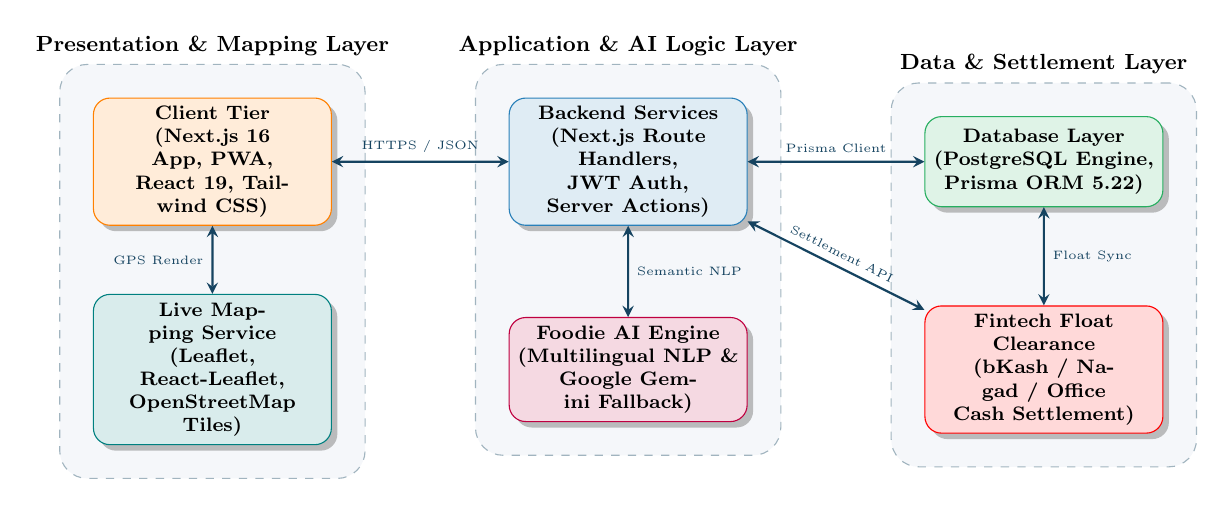
\begin{tikzpicture}[
        scale=0.88, transform shape,
        box/.style={draw=tikzborder, fill=white, rounded corners=6pt, text width=3.2cm, minimum height=1.3cm, align=center, font=\footnotesize\bfseries, drop shadow},
        layer/.style={draw=tikzdarkblue!40, fill=tikzlightgray, rounded corners=10pt, inner sep=12pt, dashed},
        arrow/.style={thick, ->, >=stealth, color=tikzdarkblue}
    ]
        % Client Tier
        \node[box, fill=orange!15, draw=orange] (client) at (0, 7.5) {Client Tier\\(Next.js 16 App, PWA,\\React 19, Tailwind CSS)};
        
        % Core API Layer
        \node[box, fill=tikzblue!15, draw=tikzblue] (api) at (6, 7.5) {Backend Services\\(Next.js Route Handlers,\\JWT Auth, Server Actions)};
        
        % Database Tier
        \node[box, fill=tikzgreen!15, draw=tikzgreen] (db) at (12, 7.5) {Database Layer\\(PostgreSQL Engine,\\Prisma ORM 5.22)};
        
        % Supporting Services
        \node[box, fill=purple!15, draw=purple] (ai) at (6, 4.5) {Foodie AI Engine\\(Multilingual NLP \&\\Google Gemini Fallback)};
        
        \node[box, fill=teal!15, draw=teal] (maps) at (0, 4.5) {Live Mapping Service\\(Leaflet, React-Leaflet,\\OpenStreetMap Tiles)};
        
        \node[box, fill=red!15, draw=red] (fintech) at (12, 4.5) {Fintech Float Clearance\\(bKash / Nagad / Office\\Cash Settlement)};

        % Background Container Layers
        \begin{scope}[on background layer]
            \node[layer, fit=(client)(maps), label=above:{\textbf{\small Presentation \& Mapping Layer}}] {};
            \node[layer, fit=(api)(ai), label=above:{\textbf{\small Application \& AI Logic Layer}}] {};
            \node[layer, fit=(db)(fintech), label=above:{\textbf{\small Data \& Settlement Layer}}] {};
        \end{scope}

        % Connecting Arrows
        \draw[arrow, <->] (client) -- node[above, font=\tiny] {HTTPS / JSON} (api);
        \draw[arrow, <->] (api) -- node[above, font=\tiny] {Prisma Client} (db);
        \draw[arrow, <->] (client) -- node[left, font=\tiny] {GPS Render} (maps);
        \draw[arrow, <->] (api) -- node[right, font=\tiny] {Semantic NLP} (ai);
        \draw[arrow, <->] (db) -- node[right, font=\tiny] {Float Sync} (fintech);
        \draw[arrow, <->] (api) -- node[above, font=\tiny, sloped] {Settlement API} (fintech);
    \end{tikzpicture}
    \caption{FoodDrop System Architecture}
    \label{fig:architecture}
\end{figure}

\begin{table}[h!]
\centering
\caption{Core Data Models}
\label{tab:data_models}
\begin{tabular}{|l|p{11cm}|}
\hline
\textbf{Model} & \textbf{Purpose} \\
\hline
User & Authentication, roles (Customer, Restaurant Owner, Rider), rating, balance \\
\hline
Restaurant & Restaurant/Home-kitchen profile, owner relation, active status \\
\hline
MenuItem & Dish details, pricing, discount tags, category, availability \\
\hline
Order & Total amount, delivery fee, 5-stage status, customer/rider linkage \\
\hline
OrderItem & Line items, quantity, item price snapshot \\
\hline
Settlement & Rider COD cash deposits (bKash/Nagad/Office), transaction IDs \\
\hline
PasswordReset & 6-digit OTP codes, email reference, 10-minute expiry timestamps \\
\hline
\end{tabular}
\end{table}

\newpage

% ---------------------------------------------------------
% Figure 3.2: Use Case Diagram (Native TikZ Diagram)
% ---------------------------------------------------------
\subsection{Use Case Diagram}
Figure \ref{fig:use_case} illustrates the use cases executable by Customers, Restaurant Owners, Delivery Riders, and Platform Administrators.

\begin{figure}[h!]
    \centering
    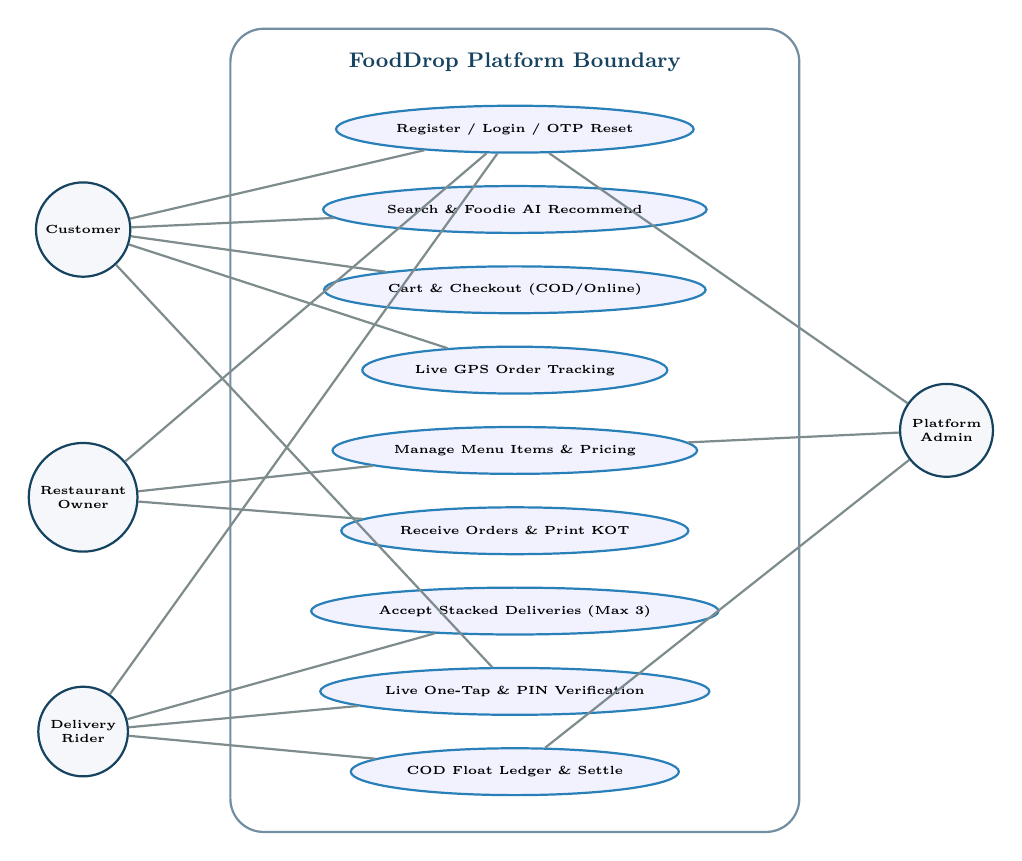
\begin{tikzpicture}[
        scale=0.85, transform shape,
        actor/.style={draw=tikzdarkblue, fill=tikzlightgray, thick, shape=circle, minimum size=0.8cm, font=\bfseries\tiny, align=center},
        usecase/.style={draw=tikzblue, fill=blue!5, thick, ellipse, minimum width=3.8cm, minimum height=0.7cm, align=center, font=\tiny\bfseries},
        system/.style={draw=tikzdarkblue!60, fill=white, rounded corners=12pt, thick}
    ]
        % System Boundary
        \draw[system] (0,-0.5) rectangle (8.5, 11.5);
        \node[font=\small\bfseries, color=tikzdarkblue] at (4.25, 11.0) {FoodDrop Platform Boundary};

        % Actors
        \node[actor] (cust) at (-2.2, 8.5) {Customer};
        \node[actor] (owner) at (-2.2, 4.5) {Restaurant\\Owner};
        \node[actor] (rider) at (-2.2, 1.0) {Delivery\\Rider};
        \node[actor] (admin) at (10.7, 5.5) {Platform\\Admin};

        % Use Cases
        \node[usecase] (uc1) at (4.25, 10.0) {Register / Login / OTP Reset};
        \node[usecase] (uc2) at (4.25, 8.8) {Search \& Foodie AI Recommend};
        \node[usecase] (uc3) at (4.25, 7.6) {Cart \& Checkout (COD/Online)};
        \node[usecase] (uc4) at (4.25, 6.4) {Live GPS Order Tracking};
        \node[usecase] (uc5) at (4.25, 5.2) {Manage Menu Items \& Pricing};
        \node[usecase] (uc6) at (4.25, 4.0) {Receive Orders \& Print KOT};
        \node[usecase] (uc7) at (4.25, 2.8) {Accept Stacked Deliveries (Max 3)};
        \node[usecase] (uc8) at (4.25, 1.6) {Live One-Tap \& PIN Verification};
        \node[usecase] (uc9) at (4.25, 0.4) {COD Float Ledger \& Settle};

        % Associations
        \draw[thick, draw=tikzgray] (cust) -- (uc1);
        \draw[thick, draw=tikzgray] (cust) -- (uc2);
        \draw[thick, draw=tikzgray] (cust) -- (uc3);
        \draw[thick, draw=tikzgray] (cust) -- (uc4);
        \draw[thick, draw=tikzgray] (cust) -- (uc8);

        \draw[thick, draw=tikzgray] (owner) -- (uc1);
        \draw[thick, draw=tikzgray] (owner) -- (uc5);
        \draw[thick, draw=tikzgray] (owner) -- (uc6);

        \draw[thick, draw=tikzgray] (rider) -- (uc1);
        \draw[thick, draw=tikzgray] (rider) -- (uc7);
        \draw[thick, draw=tikzgray] (rider) -- (uc8);
        \draw[thick, draw=tikzgray] (rider) -- (uc9);

        \draw[thick, draw=tikzgray] (admin) -- (uc1);
        \draw[thick, draw=tikzgray] (admin) -- (uc5);
        \draw[thick, draw=tikzgray] (admin) -- (uc9);
    \end{tikzpicture}
    \caption{Use Case Diagram of FoodDrop}
    \label{fig:use_case}
\end{figure}

\newpage

% ---------------------------------------------------------
% Figure 3.3: Context Level Diagram (DFD-0) (Native TikZ Diagram)
% ---------------------------------------------------------
\subsection{Context Level Diagram (DFD-0)}
Figure \ref{fig:dfd0} depicts the Context-Level Data Flow Diagram (DFD Level 0) representing the external entities interacting with FoodDrop.

\begin{figure}[h!]
    \centering
    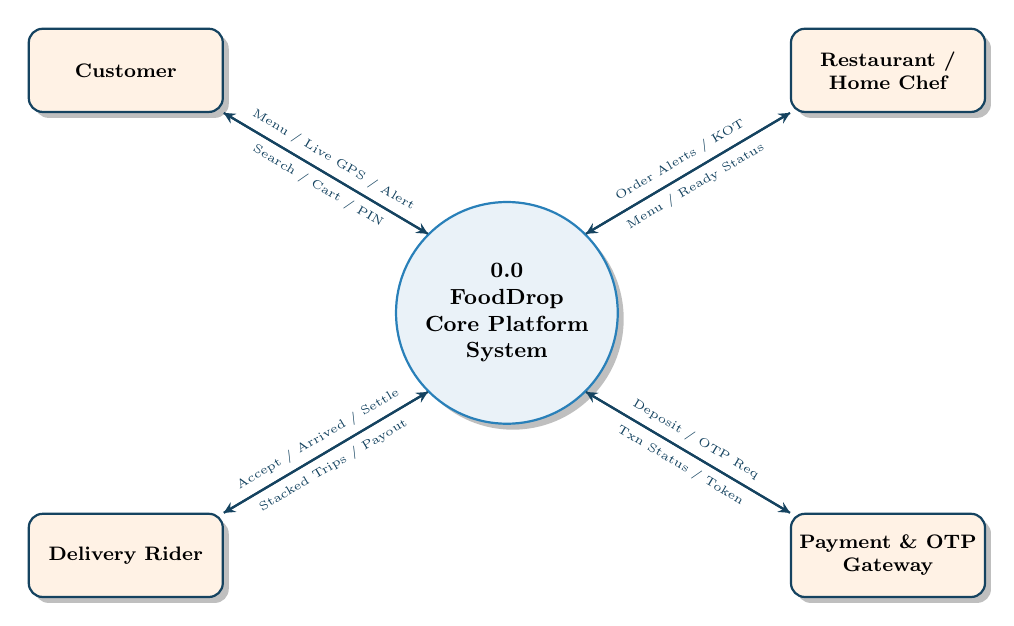
\begin{tikzpicture}[
        scale=0.88, transform shape,
        process/.style={draw=tikzblue, fill=tikzblue!10, thick, circle, minimum size=3.2cm, align=center, font=\small\bfseries, drop shadow},
        entity/.style={draw=tikzdarkblue, fill=orange!10, thick, rectangle, rounded corners=5pt, minimum width=2.8cm, minimum height=1.2cm, align=center, font=\footnotesize\bfseries, drop shadow},
        arrow/.style={thick, ->, >=stealth, color=tikzdarkblue}
    ]
        % Central Process
        \node[process] (system) at (0, 0) {0.0\\FoodDrop\\Core Platform\\System};

        % External Entities
        \node[entity] (cust) at (-5.5, 3.5) {Customer};
        \node[entity] (owner) at (5.5, 3.5) {Restaurant /\\Home Chef};
        \node[entity] (rider) at (-5.5, -3.5) {Delivery Rider};
        \node[entity] (gateway) at (5.5, -3.5) {Payment \& OTP\\Gateway};

        % Data Flows - Customer
        \draw[arrow] (cust.south east) -- node[below, font=\tiny, sloped] {Search / Cart / PIN} (system.north west);
        \draw[arrow] (system.north west) -- node[above, font=\tiny, sloped] {Menu / Live GPS / Alert} (cust.south east);

        % Data Flows - Restaurant
        \draw[arrow] (owner.south west) -- node[below, font=\tiny, sloped] {Menu / Ready Status} (system.north east);
        \draw[arrow] (system.north east) -- node[above, font=\tiny, sloped] {Order Alerts / KOT} (owner.south west);

        % Data Flows - Rider
        \draw[arrow] (rider.north east) -- node[above, font=\tiny, sloped] {Accept / Arrived / Settle} (system.south west);
        \draw[arrow] (system.south west) -- node[below, font=\tiny, sloped] {Stacked Trips / Payout} (rider.north east);

        % Data Flows - Gateway
        \draw[arrow] (system.south east) -- node[above, font=\tiny, sloped] {Deposit / OTP Req} (gateway.north west);
        \draw[arrow] (gateway.north west) -- node[below, font=\tiny, sloped] {Txn Status / Token} (system.south east);
    \end{tikzpicture}
    \caption{Context Level Diagram (DFD-0)}
    \label{fig:dfd0}
\end{figure}

% ---------------------------------------------------------
% Figure 3.4: Data Flow Diagram (DFD Level 1) (Native TikZ Diagram)
% ---------------------------------------------------------
\subsection{Data Flow Diagram (DFD Level 1)}
Figure \ref{fig:dfd1} details the functional data flow decomposed across ordering, kitchen prep, rider dispatch, and cash ledger modules.

\begin{figure}[h!]
    \centering
    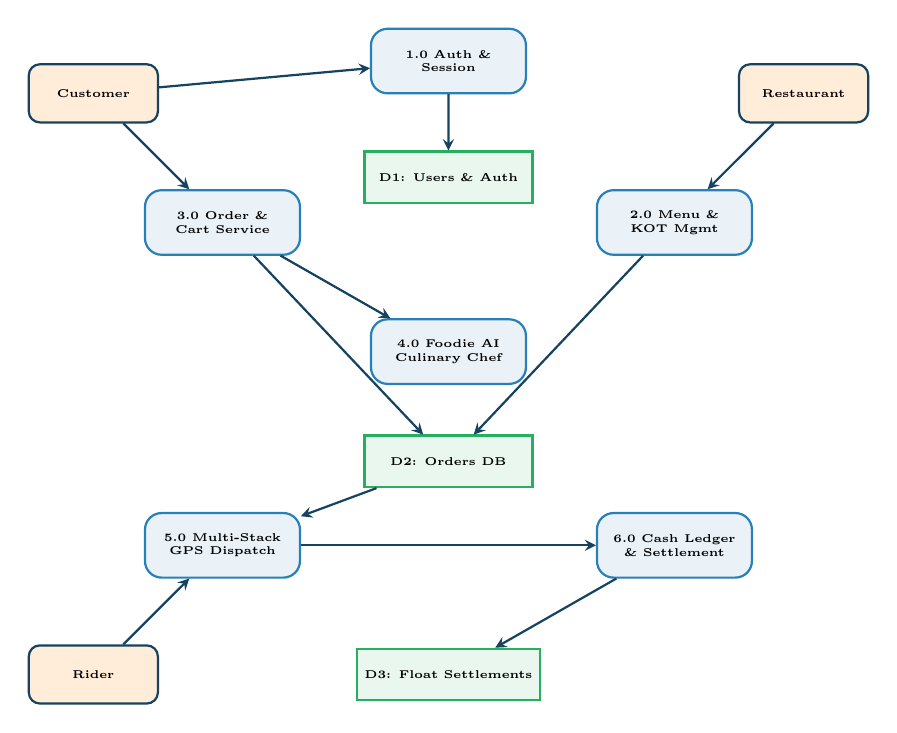
\begin{tikzpicture}[
        scale=0.82, transform shape,
        proc/.style={draw=tikzblue, fill=tikzblue!10, thick, rounded corners=6pt, minimum width=2.4cm, minimum height=1.0cm, align=center, font=\tiny\bfseries},
        store/.style={draw=tikzgreen, fill=tikzgreen!10, thick, rectangle, minimum width=2.6cm, minimum height=0.8cm, align=center, font=\tiny\bfseries},
        ent/.style={draw=tikzdarkblue, fill=orange!15, thick, rounded corners=4pt, minimum width=2.0cm, minimum height=0.9cm, align=center, font=\tiny\bfseries},
        arr/.style={thick, ->, >=stealth, color=tikzdarkblue}
    ]
        % Entities
        \node[ent] (eCust) at (-5.5, 4.5) {Customer};
        \node[ent] (eOwner) at (5.5, 4.5) {Restaurant};
        \node[ent] (eRider) at (-5.5, -4.5) {Rider};

        % Processes
        \node[proc] (pAuth) at (0, 5.0) {1.0 Auth \&\\Session};
        \node[proc] (pMenu) at (3.5, 2.5) {2.0 Menu \&\\KOT Mgmt};
        \node[proc] (pOrder) at (-3.5, 2.5) {3.0 Order \&\\Cart Service};
        \node[proc] (pAI) at (0, 0.5) {4.0 Foodie AI\\Culinary Chef};
        \node[proc] (pRider) at (-3.5, -2.5) {5.0 Multi-Stack\\GPS Dispatch};
        \node[proc] (pSettle) at (3.5, -2.5) {6.0 Cash Ledger\\\& Settlement};

        % Data Stores
        \node[store] (dUser) at (0, 3.2) {D1: Users \& Auth};
        \node[store] (dOrder) at (0, -1.2) {D2: Orders DB};
        \node[store] (dSettle) at (0, -4.5) {D3: Float Settlements};

        % Data Flow Connections
        \draw[arr] (eCust) -- (pOrder);
        \draw[arr] (pOrder) -- (dOrder);
        \draw[arr] (pOrder) -- (pAI);
        \draw[arr] (eOwner) -- (pMenu);
        \draw[arr] (pMenu) -- (dOrder);
        \draw[arr] (dOrder) -- (pRider);
        \draw[arr] (eRider) -- (pRider);
        \draw[arr] (pRider) -- (pSettle);
        \draw[arr] (pSettle) -- (dSettle);
        \draw[arr] (eCust) -- (pAuth);
        \draw[arr] (pAuth) -- (dUser);
    \end{tikzpicture}
    \caption{Data Flow Diagram --- Level 1}
    \label{fig:dfd1}
\end{figure}

\newpage

% ---------------------------------------------------------
% Figure 3.5: Database Schema (ER Diagram) (Native TikZ Diagram)
% ---------------------------------------------------------
\subsection{Database Schema (Entity-Relationship Diagram)}
Figure \ref{fig:er_diagram} displays the Entity-Relationship (ER) diagram reflecting the normalized PostgreSQL database tables.

\begin{figure}[h!]
    \centering
    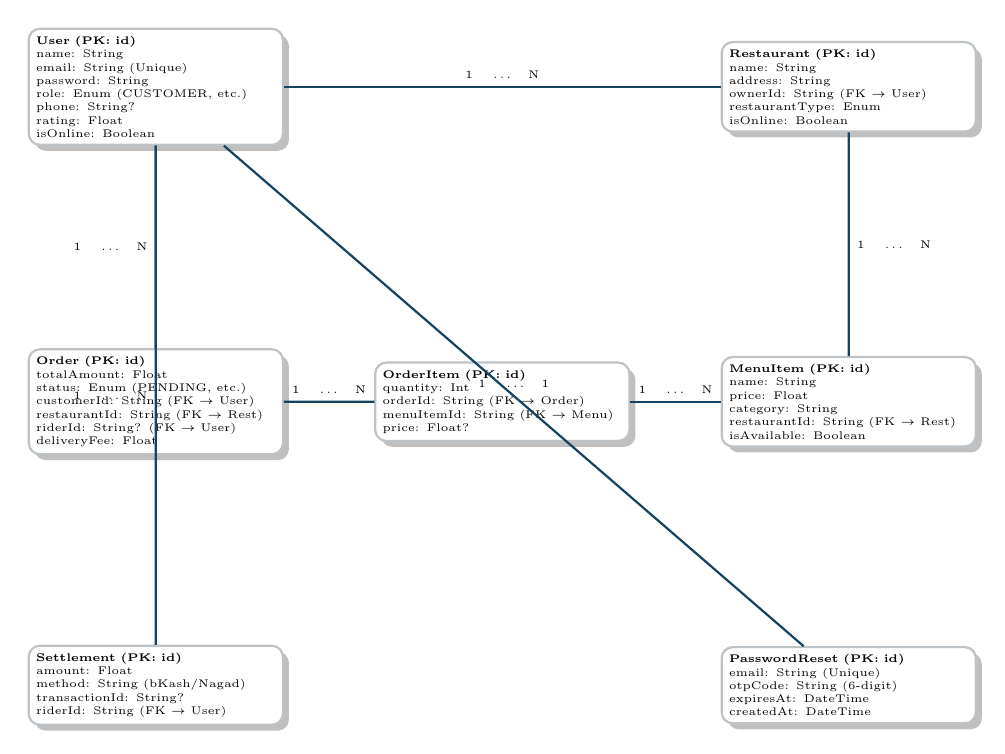
\begin{tikzpicture}[
        scale=0.80, transform shape,
        table/.style={draw=tikzborder, fill=white, thick, rounded corners=4pt, text width=3.8cm, font=\tiny, drop shadow},
        title/.style={fill=tikzblue, text=white, font=\tiny\bfseries, align=center, minimum width=3.8cm},
        rel/.style={thick, draw=tikzdarkblue}
    ]
        % User Table
        \node[table] (tbUser) at (-5.5, 4.5) {
            \textbf{User (PK: id)}\\
            name: String\\
            email: String (Unique)\\
            password: String\\
            role: Enum (CUSTOMER, etc.)\\
            phone: String?\\
            rating: Float\\
            isOnline: Boolean
        };

        % Restaurant Table
        \node[table] (tbRest) at (5.5, 4.5) {
            \textbf{Restaurant (PK: id)}\\
            name: String\\
            address: String\\
            ownerId: String (FK $\to$ User)\\
            restaurantType: Enum\\
            isOnline: Boolean
        };

        % MenuItem Table
        \node[table] (tbMenu) at (5.5, -0.5) {
            \textbf{MenuItem (PK: id)}\\
            name: String\\
            price: Float\\
            category: String\\
            restaurantId: String (FK $\to$ Rest)\\
            isAvailable: Boolean
        };

        % Order Table
        \node[table] (tbOrder) at (-5.5, -0.5) {
            \textbf{Order (PK: id)}\\
            totalAmount: Float\\
            status: Enum (PENDING, etc.)\\
            customerId: String (FK $\to$ User)\\
            restaurantId: String (FK $\to$ Rest)\\
            riderId: String? (FK $\to$ User)\\
            deliveryFee: Float
        };

        % OrderItem Table
        \node[table] (tbOrderItem) at (0, -0.5) {
            \textbf{OrderItem (PK: id)}\\
            quantity: Int\\
            orderId: String (FK $\to$ Order)\\
            menuItemId: String (FK $\to$ Menu)\\
            price: Float?
        };

        % Settlement Table
        \node[table] (tbSettle) at (-5.5, -5.0) {
            \textbf{Settlement (PK: id)}\\
            amount: Float\\
            method: String (bKash/Nagad)\\
            transactionId: String?\\
            riderId: String (FK $\to$ User)
        };

        % PasswordReset Table
        \node[table] (tbReset) at (5.5, -5.0) {
            \textbf{PasswordReset (PK: id)}\\
            email: String (Unique)\\
            otpCode: String (6-digit)\\
            expiresAt: DateTime\\
            createdAt: DateTime
        };

        % Relationships
        \draw[rel] (tbUser) -- node[above, font=\tiny] {1 \quad \dots \quad N} (tbRest);
        \draw[rel] (tbRest) -- node[right, font=\tiny] {1 \quad \dots \quad N} (tbMenu);
        \draw[rel] (tbUser) -- node[left, font=\tiny] {1 \quad \dots \quad N} (tbOrder);
        \draw[rel] (tbOrder) -- node[above, font=\tiny] {1 \quad \dots \quad N} (tbOrderItem);
        \draw[rel] (tbMenu) -- node[above, font=\tiny] {1 \quad \dots \quad N} (tbOrderItem);
        \draw[rel] (tbUser) -- node[left, font=\tiny] {1 \quad \dots \quad N} (tbSettle);
        \draw[rel] (tbUser) -- node[above, font=\tiny] {1 \quad \dots \quad 1} (tbReset);
    \end{tikzpicture}
    \caption{FoodDrop Database Schema (Entity-Relationship Diagram)}
    \label{fig:er_diagram}
\end{figure}

\newpage

% ---------------------------------------------------------
% Figure 3.6: Algorithm / Flowchart (Native TikZ Diagram)
% ---------------------------------------------------------
\subsection{Algorithm / Flowchart}
Figure \ref{fig:flowchart} outlines the sequential logic for Live Order Verification and COD Cash Settlement.

\begin{figure}[h!]
    \centering
    \begin{tikzpicture}[
        scale=0.82, transform shape,
        startstop/.style={draw=tikzred, fill=red!10, thick, rounded corners=10pt, minimum width=3.0cm, minimum height=0.8cm, align=center, font=\tiny\bfseries},
        block/.style={draw=tikzblue, fill=blue!10, thick, rectangle, rounded corners=4pt, minimum width=3.4cm, minimum height=0.8cm, align=center, font=\tiny\bfseries},
        decision/.style={draw=tikzyellow, fill=yellow!15, thick, diamond, aspect=2, minimum width=3.2cm, minimum height=0.8cm, align=center, font=\tiny\bfseries},
        arr/.style={thick, ->, >=stealth, color=tikzdarkblue}
    ]
        % Nodes
        \node[startstop] (start) at (0, 10.5) {Start Delivery Run};
        \node[block] (arrive) at (0, 9.2) {Rider Clicks "I Have Arrived"\\(Status $\to$ ARRIVED)};
        \node[decision] (online) at (0, 7.6) {Customer\\Active Online?};
        
        \node[block] (onetap) at (-3.2, 6.0) {Live Bottom-Sheet Appears\\Customer Clicks "Yes Received! 🍕"};
        \node[block] (pin) at (3.2, 6.0) {Customer Reads 4-Digit PIN\\Rider Inputs PIN in Cockpit};
        
        \node[block] (complete) at (0, 4.4) {Mark Order DELIVERED\\Trigger Confetti \& Sound};
        \node[block] (ledger) at (0, 3.2) {Update COD Float Ledger:\\$\text{Cash In Hand} = \text{Total Cash} - \text{Settled}$};
        
        \node[decision] (limit) at (0, 1.6) {Cash In Hand\\$> \text{৳}5,000$ Limit?};
        \node[block] (deposit) at (-3.2, 0.0) {Deposit Float via bKash/Nagad\\Record in Settlement Table};
        \node[startstop] (end) at (0, -1.2) {Trip Finished / Ready for Next Stack};

        % Connectors
        \draw[arr] (start) -- (arrive);
        \draw[arr] (arrive) -- (online);
        \draw[arr] (online) -- node[above, font=\tiny] {Yes} (onetap);
        \draw[arr] (online) -- node[above, font=\tiny] {No / Offline} (pin);
        \draw[arr] (onetap) |- (complete);
        \draw[arr] (pin) |- (complete);
        \draw[arr] (complete) -- (ledger);
        \draw[arr] (ledger) -- (limit);
        \draw[arr] (limit) -- node[above, font=\tiny] {Yes} (deposit);
        \draw[arr] (limit) -- node[right, font=\tiny] {No} (end);
        \draw[arr] (deposit) |- (end);
    \end{tikzpicture}
    \caption{Live One-Tap Order Verification \& Float Settlement Flowchart}
    \label{fig:flowchart}
\end{figure}

\section{Summary}
This chapter detailed the structural blueprints, technology choices, and architectural diagrams of FoodDrop. The subsequent chapter discusses the concrete implementation.

\newpage

% =========================================================
% CHAPTER 4: IMPLEMENTATION
% =========================================================
\chapter{IMPLEMENTATION}

\section{Interface / Front-End Design}
FoodDrop's frontend is constructed with React 19 and Next.js 16 using Tailwind CSS v4. Zustand provides client-side state persistence for the shopping cart. Key user interface screens include:
\begin{itemize}
    \item \textbf{Customer Discovery View:} Hero search bar with instant dish autocomplete, dual-kitchen toggle (Commercial vs. Homemade), category carousel, and food item cards with discount badges.
    \item \textbf{Cart \& Checkout Drawer:} Real-time subtotal, dynamic delivery fees, delivery address selector, and payment method options (Cash on Delivery, bKash, Nagad).
    \item \textbf{Live GPS Tracking View:} Real-time 5-stage status stepper with Leaflet OpenStreetMap visualizing restaurant, rider, and destination coordinates.
    \item \textbf{Restaurant Management Hub:} Live order board with audio alarms, KOT receipt printing, and status transitions.
    \item \textbf{Rider Cockpit:} Stacked multi-order switcher, turn-by-turn map directions, 4-digit PIN verification box, and Gamification Hub.
\end{itemize}

\section{Back-End}
The backend operates via Next.js Route Handlers and Server Actions connected to PostgreSQL via Prisma ORM:
\begin{itemize}
    \item \textbf{Strict Kitchen Preparation Lock:} In \texttt{/api/orders/rider}, validation guarantees that a rider cannot trigger \texttt{ON\_THE\_WAY} until the restaurant sets status to \texttt{READY\_FOR\_PICKUP}.
    \item \textbf{No-Cache Dynamic Streaming:} Real-time polling endpoints enforce \texttt{force-dynamic} and \texttt{revalidate = 0} to eliminate stale HTTP caching across rider and customer screens.
    \item \textbf{Authentication \& OTP Recovery:} Session tokens are signed via JWT. Password recovery is handled via a 3-step OTP pipeline (\texttt{/api/auth/forgot-password}).
\end{itemize}

\section{Modules / Features}
\begin{itemize}
    \item \textbf{Multilingual Foodie AI Chef:} Parses queries in English, Bengali, and Banglish to recommend curated dishes and combo packages with estimated calories.
    \item \textbf{Live One-Tap Confirmation:} The customer receives a prominent bottom-sheet modal upon rider arrival with backup 4-digit PIN verification.
    \item \textbf{COD Float Ledger \& Digital Settlement:} Real-time calculation of Cash in Hand, Net Rider Earnings, and Payable Balance with a ৳5,000 safety limit bar and instant bKash/Nagad settlement logging.
    \item \textbf{Rider Gamification Hub:} Tiers (Bronze, Silver, Gold, Platinum Legend), Daily Quests with claimable cash bonuses, and unlockable achievement badges.
    \item \textbf{Universal PWA Engine:} Custom service worker (\texttt{sw.js}) and web manifest (\texttt{manifest.ts}) enabling standalone app installations across iOS, Android, and Desktop.
\end{itemize}

\section{Summary}
This chapter detailed the frontend, backend, and domain-specific logic implementations. The next chapter provides the user manual.

\newpage

% =========================================================
% CHAPTER 5: USER MANUAL
% =========================================================
\chapter{USER MANUAL}

\section{System Requirement}

\subsection{Hardware Requirement}
\begin{itemize}
    \item \textbf{Client Device:} Any modern smartphone, tablet, laptop, or desktop with an active internet connection.
    \item \textbf{Server / Development Machine:} Minimum 4 GB RAM (8 GB recommended), Dual-Core Processor, 500 MB free storage.
\end{itemize}

\subsection{Software Requirement}
\begin{itemize}
    \item \textbf{Operating System:} Windows 10/11, macOS, Linux, Android, or iOS.
    \item \textbf{Browser:} Google Chrome (v110+), Mozilla Firefox, Apple Safari, or Microsoft Edge.
    \item \textbf{Runtime Environment:} Node.js v18.18+ / v20+.
    \item \textbf{Database:} PostgreSQL (Supabase / Local).
\end{itemize}

\section{User Interfaces}

% ---------------------------------------------------------
% UI Screenshot Placeholders (You can simply upload your image files)
% ---------------------------------------------------------
\begin{figure}[h!]
    \centering
    \IfFileExists{figure_5_1_customer_homepage.png}{
        \includegraphics[width=0.85\textwidth]{figure_5_1_customer_homepage.png}
    }{
        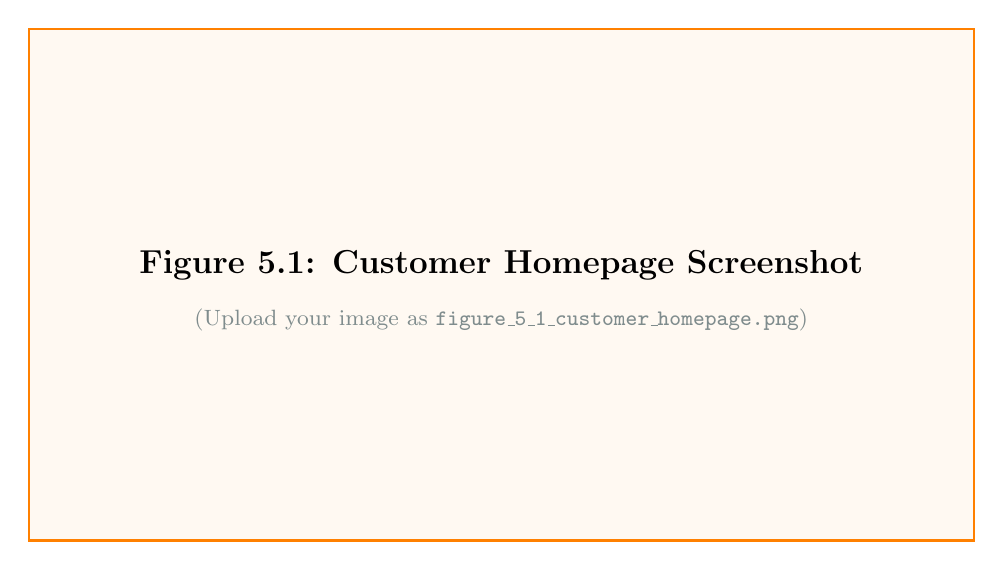
\begin{tikzpicture}
            \draw[thick, fill=orange!5, draw=orange] (0,0) rectangle (12, 6.5);
            \node at (6, 3.5) {\textbf{\large Figure 5.1: Customer Homepage Screenshot}};
            \node[font=\footnotesize, text=tikzgray] at (6, 2.8) {(Upload your image as \texttt{figure\_5\_1\_customer\_homepage.png})};
        \end{tikzpicture}
    }
    \caption{Customer Homepage --- Dish Search, Categories, and Kitchen Filter}
    \label{fig:ui_home}
\end{figure}

\begin{figure}[h!]
    \centering
    \IfFileExists{figure_5_2_ai_chef_assistant.png}{
        \includegraphics[width=0.8\textwidth]{figure_5_2_ai_chef_assistant.png}
    }{
        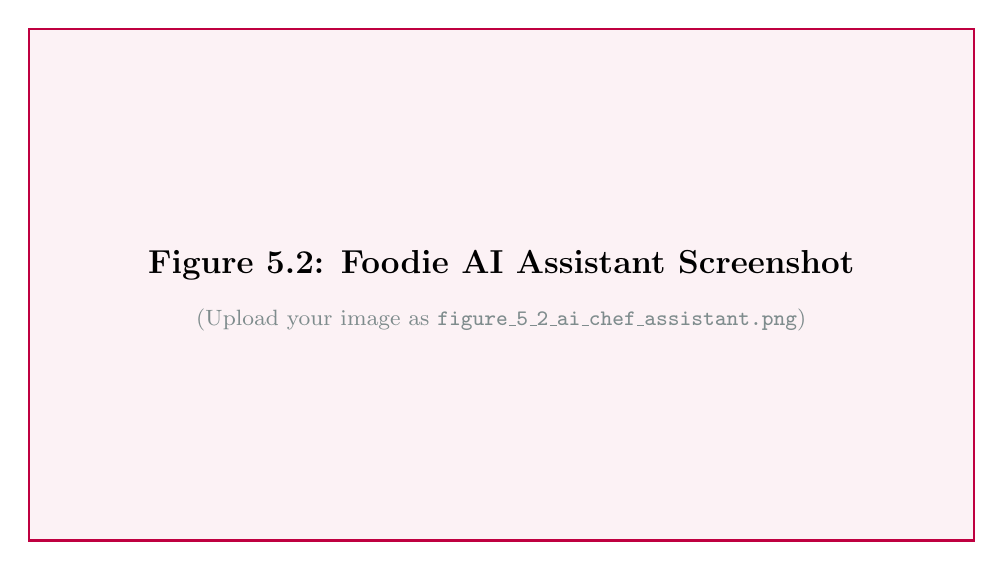
\begin{tikzpicture}
            \draw[thick, fill=purple!5, draw=purple] (0,0) rectangle (12, 6.5);
            \node at (6, 3.5) {\textbf{\large Figure 5.2: Foodie AI Assistant Screenshot}};
            \node[font=\footnotesize, text=tikzgray] at (6, 2.8) {(Upload your image as \texttt{figure\_5\_2\_ai\_chef\_assistant.png})};
        \end{tikzpicture}
    }
    \caption{Foodie AI Culinary Assistant --- Multilingual Recommendation Prompt}
    \label{fig:ui_ai}
\end{figure}

\newpage

\begin{figure}[h!]
    \centering
    \IfFileExists{figure_5_3_order_tracking_gps.png}{
        \includegraphics[width=0.85\textwidth]{figure_5_3_order_tracking_gps.png}
    }{
        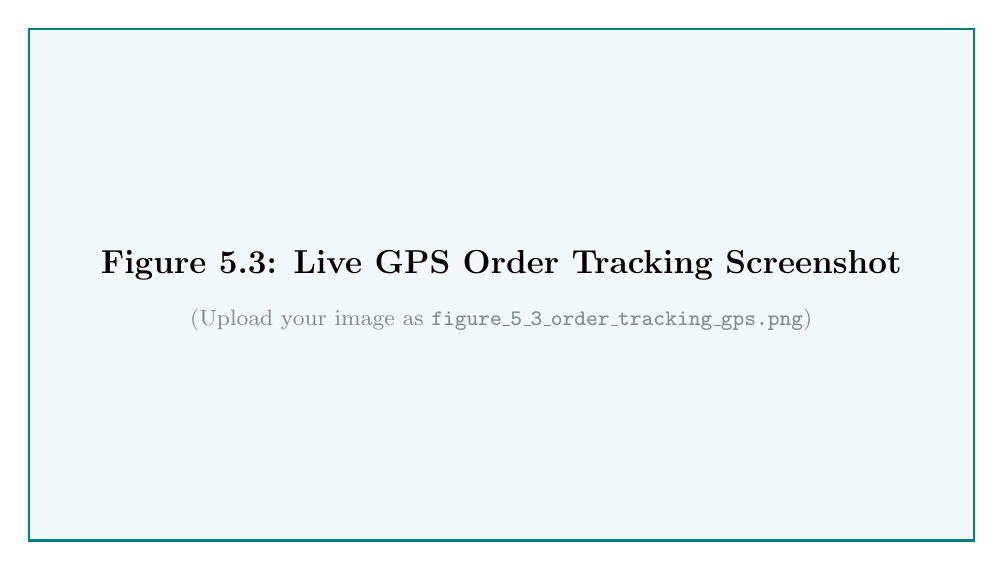
\begin{tikzpicture}
            \draw[thick, fill=teal!5, draw=teal] (0,0) rectangle (12, 6.5);
            \node at (6, 3.5) {\textbf{\large Figure 5.3: Live GPS Order Tracking Screenshot}};
            \node[font=\footnotesize, text=tikzgray] at (6, 2.8) {(Upload your image as \texttt{figure\_5\_3\_order\_tracking\_gps.png})};
        \end{tikzpicture}
    }
    \caption{Live GPS Order Tracking View with Arrival Confirmation Card}
    \label{fig:ui_track}
\end{figure}

\begin{figure}[h!]
    \centering
    \IfFileExists{figure_5_4_restaurant_dashboard.png}{
        \includegraphics[width=0.85\textwidth]{figure_5_4_restaurant_dashboard.png}
    }{
        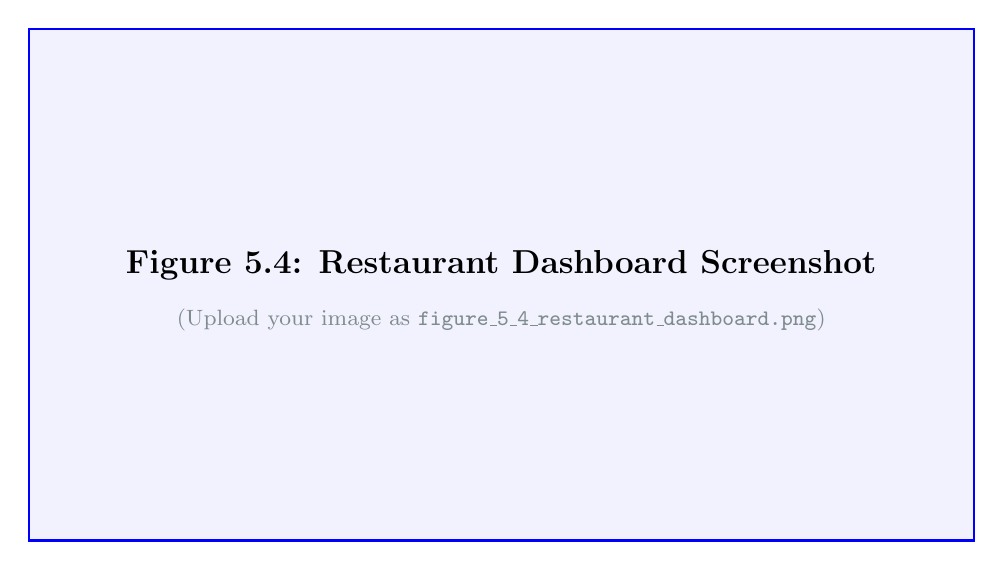
\begin{tikzpicture}
            \draw[thick, fill=blue!5, draw=blue] (0,0) rectangle (12, 6.5);
            \node at (6, 3.5) {\textbf{\large Figure 5.4: Restaurant Dashboard Screenshot}};
            \node[font=\footnotesize, text=tikzgray] at (6, 2.8) {(Upload your image as \texttt{figure\_5\_4\_restaurant\_dashboard.png})};
        \end{tikzpicture}
    }
    \caption{Restaurant Dashboard --- Incoming Orders and KOT Printing}
    \label{fig:ui_rest}
\end{figure}

\newpage

\begin{figure}[h!]
    \centering
    \IfFileExists{figure_5_5_rider_cockpit.png}{
        \includegraphics[width=0.85\textwidth]{figure_5_5_rider_cockpit.png}
    }{
        \begin{tikzpicture}
            \draw[thick, fill=amber!5, draw=amber] (0,0) rectangle (12, 6.5);
            \node at (6, 3.5) {\textbf{\large Figure 5.5: Rider Delivery Cockpit Screenshot}};
            \node[font=\footnotesize, text=tikzgray] at (6, 2.8) {(Upload your image as \texttt{figure\_5\_5\_rider\_cockpit.png})};
        \end{tikzpicture}
    }
    \caption{Rider Delivery Cockpit --- Stacked Trips and Navigation Map}
    \label{fig:ui_rider}
\end{figure}

\begin{figure}[h!]
    \centering
    \IfFileExists{figure_5_6_rider_gamification_ledger.png}{
        \includegraphics[width=0.85\textwidth]{figure_5_6_rider_gamification_ledger.png}
    }{
        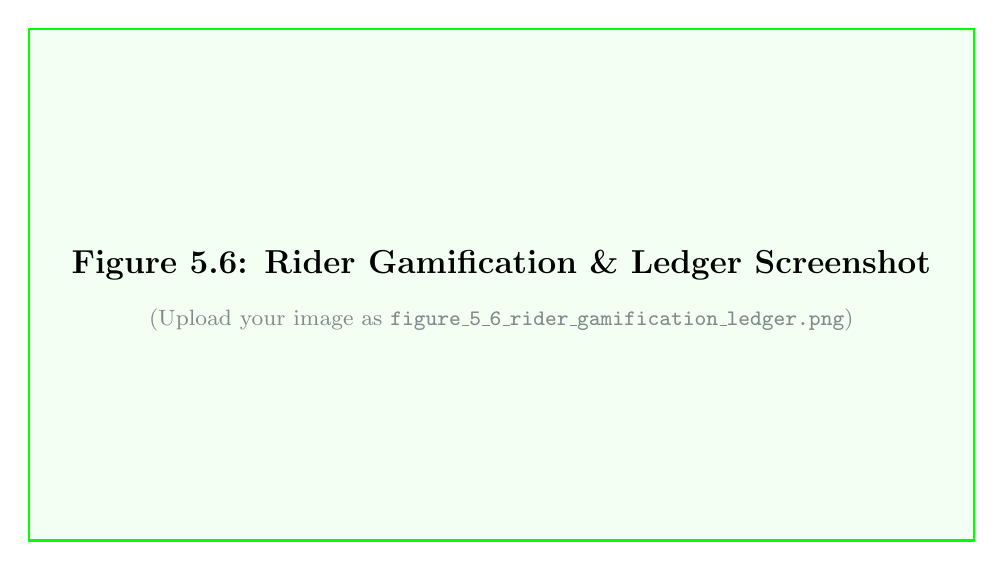
\begin{tikzpicture}
            \draw[thick, fill=green!5, draw=green] (0,0) rectangle (12, 6.5);
            \node at (6, 3.5) {\textbf{\large Figure 5.6: Rider Gamification \& Ledger Screenshot}};
            \node[font=\footnotesize, text=tikzgray] at (6, 2.8) {(Upload your image as \texttt{figure\_5\_6\_rider\_gamification\_ledger.png})};
        \end{tikzpicture}
    }
    \caption{Rider Gamification Hub, Float Ledger \& Digital Settlement Modal}
    \label{fig:ui_ledger}
\end{figure}

\subsection{Login Credentials}
For evaluation, sample seeded accounts are available (password: \texttt{password123}):
\begin{table}[h!]
\centering
\begin{tabular}{|l|l|}
\hline
\textbf{Role} & \textbf{Email Address} \\
\hline
Customer & \texttt{customer@fooddrop.com} \\
\hline
Restaurant Owner & \texttt{owner@fooddrop.com} \\
\hline
Delivery Rider & \texttt{rider@fooddrop.com} \\
\hline
\end{tabular}
\end{table}

\section{Discussion}
The integration of live one-tap confirmations and the COD float ledger solves core trust and cash-handling issues prevalent in local delivery operations. Moreover, the lightweight NLP fallback ensures uninterrupted meal recommendations regardless of external API quotas.

\newpage

% =========================================================
% CHAPTER 6: CONCLUSION
% =========================================================
\chapter{CONCLUSION}

\section{Conclusion}
FoodDrop demonstrates that a modern food delivery platform can integrate artificial intelligence, multi-order logistics, and fintech clearance into a seamless web and PWA application. By combining strict type safety (TypeScript), reactive client state (Zustand), and reliable persistence (Prisma ORM \& PostgreSQL), FoodDrop provides an enterprise-ready foundation for hyper-local food commerce.

\section{Limitations}
\begin{itemize}
    \item High-traffic real-time GPS tracking currently relies on interval polling rather than dedicated WebSockets.
    \item AI food recommendations depend on structured menu item descriptions provided by restaurant owners.
    \item Native biometric authentication (FaceID/Fingerprint) is not directly integrated into the web layer.
\end{itemize}

\section{Future Works}
\begin{itemize}
    \item Implement real-time WebSocket communication for instantaneous GPS coordinates and chat streaming.
    \item Integrate automated online payment gateways (SSLCommerz, bKash Direct Checkout API).
    \item Develop native mobile applications using React Native / Flutter sharing the same backend APIs.
    \item Expand AI Chef to interpret uploaded dish photographs for calorie estimation and reverse recipe discovery.
\end{itemize}

\newpage

% =========================================================
% REFERENCES
% =========================================================
\chapter*{REFERENCES}
\addcontentsline{toc}{chapter}{References}

\noindent [1] Next.js Documentation. Vercel Inc., 2026. \url{https://nextjs.org/docs}

\noindent [2] React 19 Official Documentation. Meta Platforms, Inc., 2026. \url{https://react.dev/}

\noindent [3] Prisma ORM Documentation. Prisma Data, Inc., 2026. \url{https://www.prisma.io/docs}

\noindent [4] Leaflet - An Open-Source JavaScript Library for Mobile-Friendly Interactive Maps. \url{https://leafletjs.com/}

\noindent [5] Google Gemini API Documentation. Google AI for Developers, 2026. \url{https://ai.google.dev/}

\noindent [6] Progressive Web Apps (PWA) Documentation. MDN Web Docs, 2026. \url{https://developer.mozilla.org/en-US/docs/Web/Progressive_web_apps}

\newpage

% =========================================================
% APPENDIX A: CODE EXCERPTS
% =========================================================
\chapter*{APPENDIX A: REPRESENTATIVE CODE EXCERPTS}
\addcontentsline{toc}{chapter}{Appendix A: Representative Code Excerpts}

This appendix provides representative implementation excerpts from the FoodDrop codebase.

\subsection*{A.1 Rider COD Float Settlement API}
\begin{lstlisting}[language=Java]
// src/app/api/rider/settle/route.ts
export async function POST(request: Request) {
  const { riderId, amount, method, transactionId } = await request.json();
  const numAmount = parseFloat(amount);

  const allDelivered = await prisma.order.findMany({
    where: { riderId, status: "DELIVERED" }
  });
  const grossCash = allDelivered.reduce((sum, o) => sum + o.totalAmount, 0);
  const earnings = allDelivered.reduce((sum, o) => sum + (o.deliveryFee || 60), 0);
  
  const settlements = await prisma.settlement.findMany({ where: { riderId } });
  const totalSettled = settlements.reduce((sum, s) => sum + s.amount, 0);
  const payable = Math.max(0, grossCash - earnings - totalSettled);

  if (numAmount > payable) {
    return NextResponse.json({ message: "Deposit exceeds payable balance!" }, { status: 400 });
  }

  const settlement = await prisma.settlement.create({
    data: { riderId, amount: numAmount, method: method || "BKASH", transactionId }
  });

  return NextResponse.json({ success: true, settlement, remainingPayable: payable - numAmount });
}
\end{lstlisting}

\subsection*{A.2 Kitchen Lock Status Validation}
\begin{lstlisting}[language=Java]
// src/app/api/orders/rider/route.ts
if (status === "ON_THE_WAY") {
  const existingOrder = await prisma.order.findUnique({ where: { id: orderId } });
  if (existingOrder.status !== "READY_FOR_PICKUP") {
    return NextResponse.json(
      { message: "Food is still being prepared by the kitchen!" },
      { status: 400 }
    );
  }
}
\end{lstlisting}

\end{document}
